\documentclass{article}

\usepackage[final]{neurips_2019}

\usepackage[utf8]{inputenc}
\usepackage[T1]{fontenc}
\usepackage{hyperref}
\usepackage{url}
\usepackage{booktabs}
\usepackage{amsfonts}
\usepackage{amsmath, bm, bbm}
\usepackage{amssymb}
\usepackage{nicefrac}
\usepackage{microtype}
\usepackage{graphicx}
\usepackage{xcolor}
\usepackage{lipsum}
\usepackage{makecell}

\newcommand{\note}[1]{\textcolor{blue}{{#1}}}

\title{
  Title of your project \\
  \vspace{1em}
  \small{\normalfont Stanford CS224N Default Project}  % Select one and delete the other
}

\author{
  Joseph Pagadora, $\;$ Steve Gan \\
  Stanford University \\
  \texttt{jcp737@stanford.edu}$\;\;\;\;$
  \texttt{zgan@stanford.edu} \\
  % Examples of more authors
%   \And
%   Name \\
%   Department of Computer Science \\
%   Stanford University \\
%   \texttt{name@stanford.edu} \\
%   \And
%   Name \\
%   Department of Computer Science \\
%   Stanford University \\
%   \texttt{name@stanford.edu}
}

\begin{document}

\maketitle

% \begin{abstract}
%   Required for final report
% \end{abstract}

\section{Research paper summary}

\begin{table}[h]
    \centering
    \begin{tabular}{ll}
        \toprule
        \textbf{Title} & \makecell{QANet: Combining Local Convolution with Global Self-Attention for \\ Reading Comprehension} \\
        \midrule
        \textbf{Authors} & \makecell{Adams Wei Yu, David Dohan, Minh-Thang Luong, Rui Zhao, \\ Kai Chen, Mohammad Norouzi, Quoc V. Le} \\
        \textbf{Venue} & ICLR 2018 \\
        \textbf{Year}  & 2018 \\
        \textbf{URL}   & \url{https://arxiv.org/pdf/1804.09541.pdf} \\
        \bottomrule
    \end{tabular}
    \vspace{1em}
\end{table}

\paragraph{Background.}
This paper introduces a new approach to reading comprehension and question-answering completely without the use of RNNs. Many of the prior works toward this problems involve the use of RNNs and their ability to encode sequential data, but as a consequence, this results in longer training and inference. At the time that RNNs in addition to attention were the best way to learn from language data, but this paper instead uses convolutional layers with self-attention in order to perform the task of question-answering with much faster training and inference times.

\begin{figure}[h]
\centering
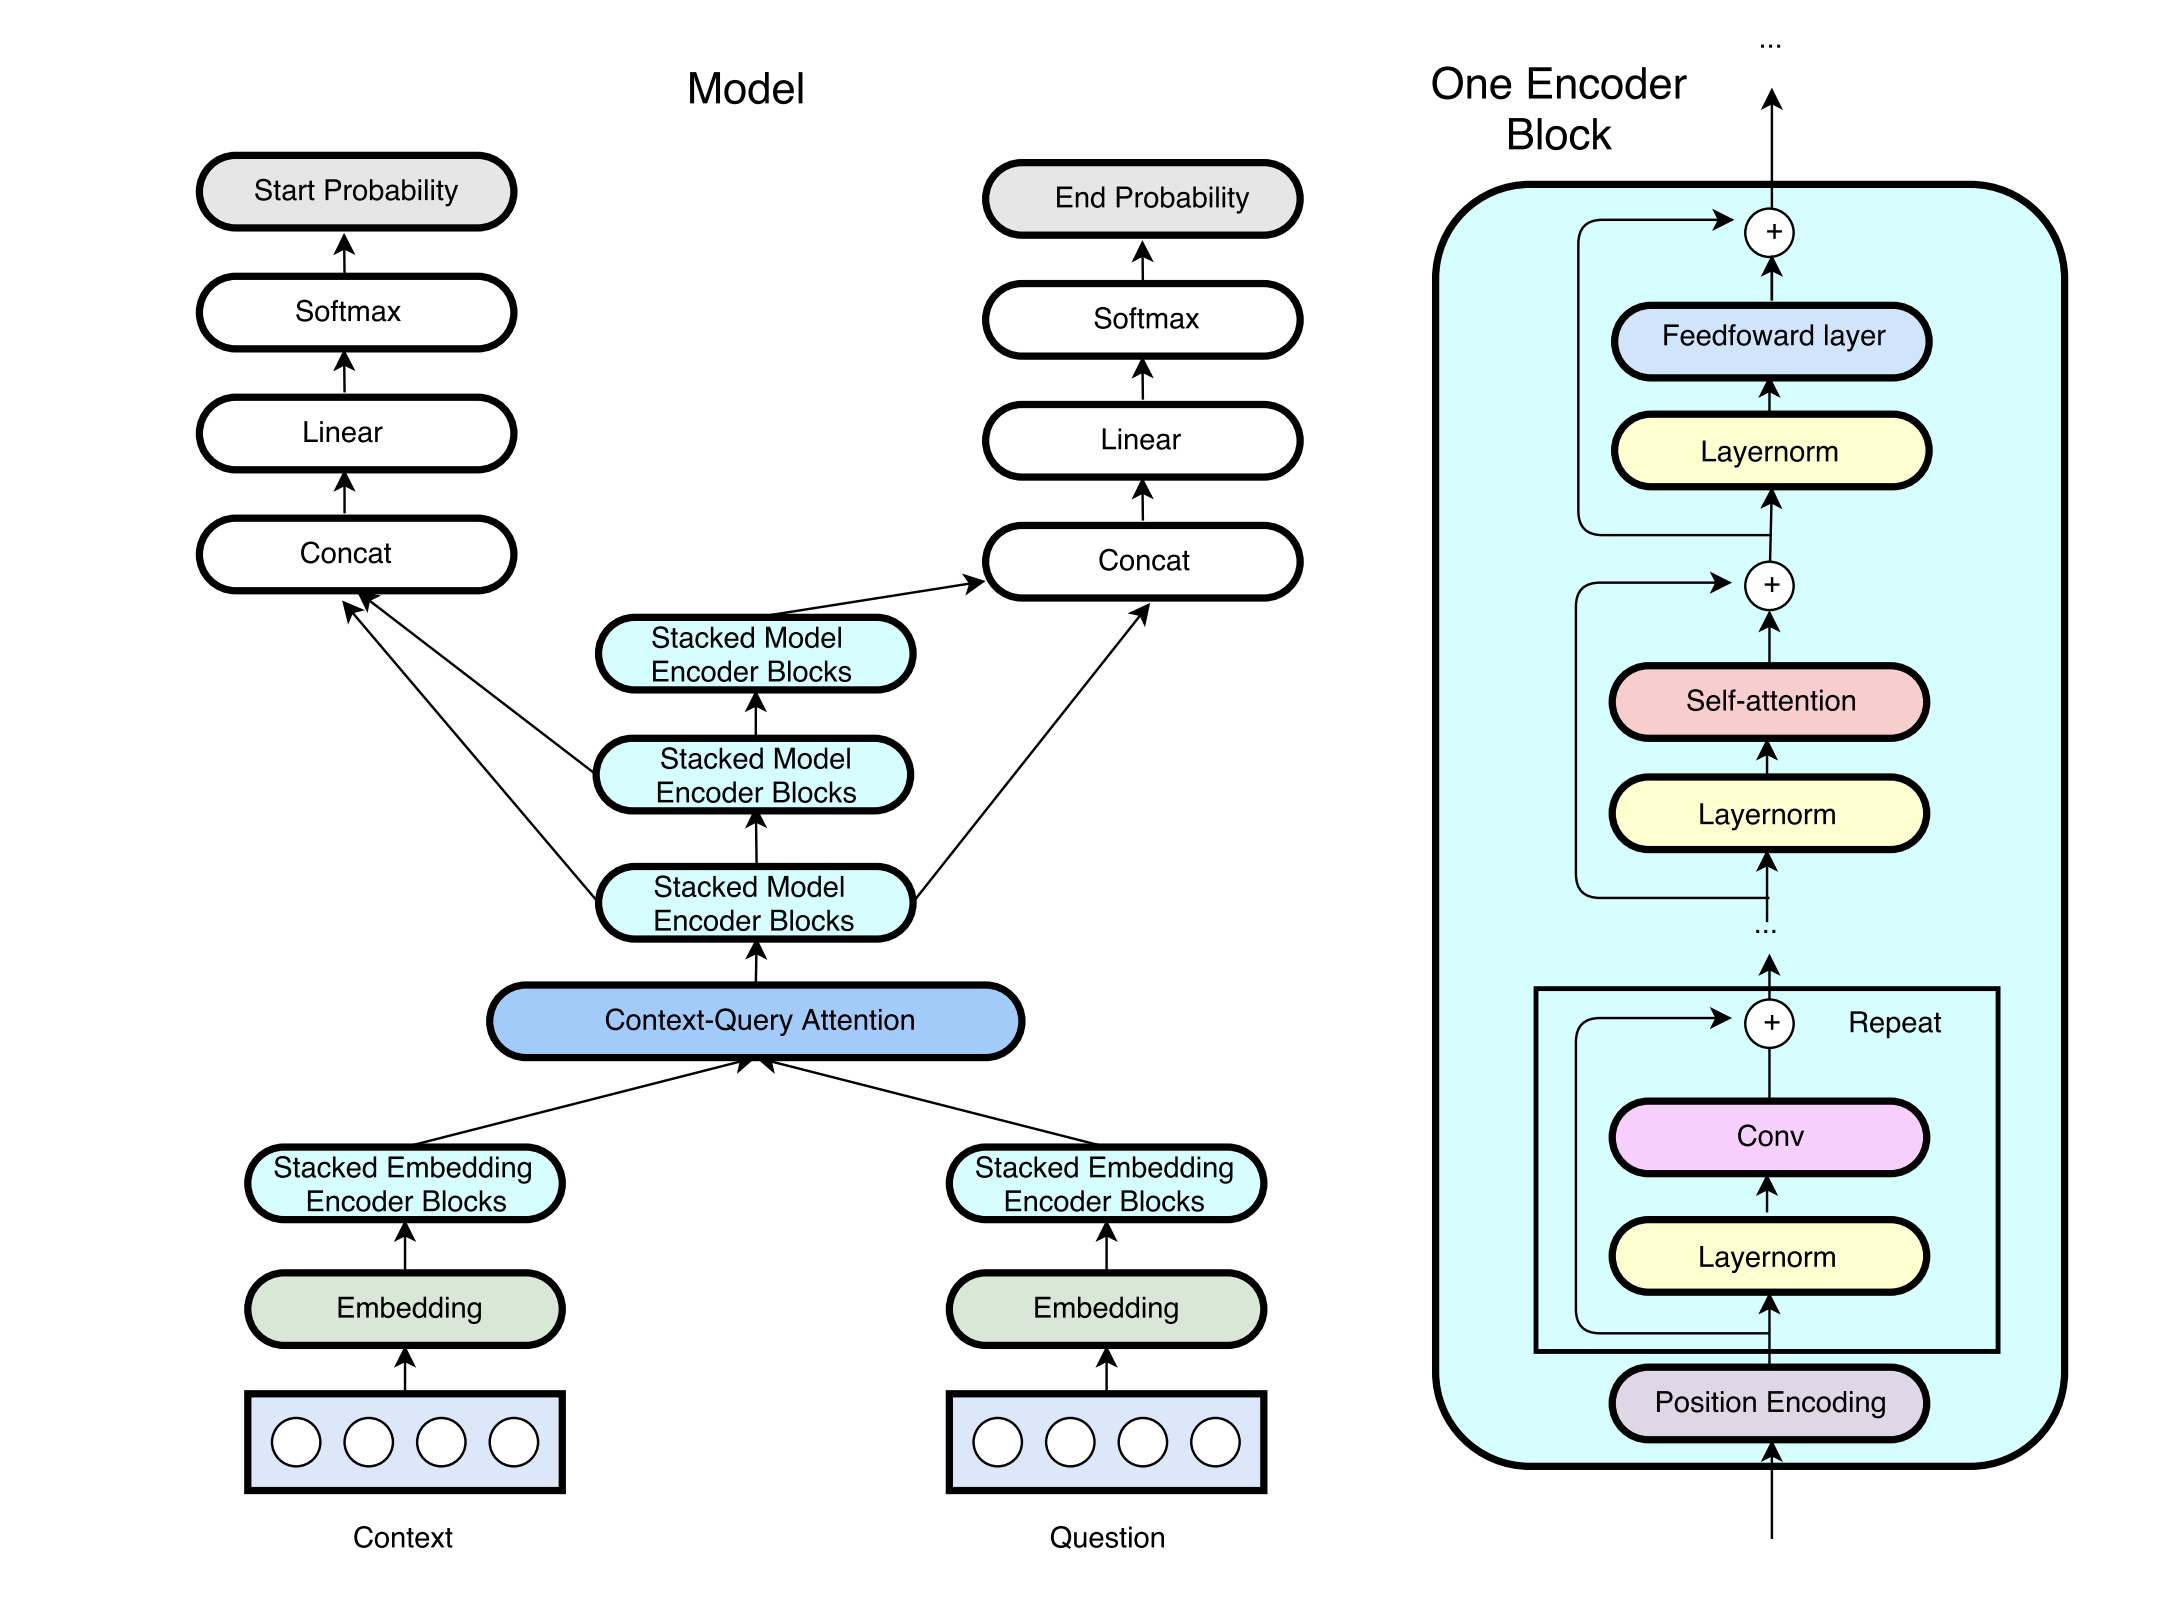
\includegraphics[scale=0.3]{model_diagram}
\caption{Left: Architecture of QANet with convolution and self-attention. Right: Encoder block that is used throughout the model}
\end{figure}

\paragraph{Summary of contributions.}
This paper proposes a new and faster way to approach the task of reading comprehension and question-answering without the use of a recurrent model, motivated by slow training and inference of such as model. The paper outlines a new method of using encoders consisting only of convolutional layers for local analysis of the input, along with self-attention for a global analysis, in order to perform the task at hand. This resulted in an increase in training speed of about 3 to 13 times and in inference speed of about 4 to 9 times faster than previous high-accuracy methods that use RNNs. \\
Because of this drastic increase in efficiency, the model is able to be trained on a much larger dataset. Using the SQuAD dataset, they also devised a data-augmentation approach by esse,ntially taking the data, translating it to another language, and then translating it back to English. Obviously, they hoped for an imperfect translator, i.e., one that does not provide an invertible mapping. That is, the synthesized datapoint has different phrasing than the original. This technique allows the model to be trained on even more data thus improving performance on the task. The authors were able to achieve a 84.6 F1 score on the SQuAD test set after training on the augmented SQuAD training set. \\
The model is outlined in detail in the paper, but Figure 1 shows a summarized diagram of the architecture of QANet. The raw input is given as $(C,Q)=$ (context, question) pairs, where the context $C=\{c_1,...,c_n\}$ consists of, say, $n$ words, and the model is to output a consecutive span $S=\{c_s,...,c_e\}\subseteq C$ containing the answer to question $Q.$ The QANet model itself outputs softmax probabilities of each word in the context being the start and end positions $s,e,$ respectively. The first step is to embed the context and question using standard embedding procedures such as GloVe. Then, these embeddings are put through multiple embedding encoder blocks. Figure 1 shows that each encoder block consists of three residual blocks, each containing a convolutional layer, a self-attention layer, and a feed-forward layer, in order. Then, the encoded context and question are put through a standard context-query attention layer. After this, the attention output is put through three model encoders $M_0, M_1,$ and $M_2.$ With learnable parameters $W_0$ and $W_1,$ each position $i$ in the context is given a start and end probability
$$p_1(i)=\text{softmax}(W_1[M_0;M_1]),\;\;\;\; p_2(i)=\text{softmax}(W_2[M_0;M_2]),$$
where $[\cdot \;; \cdot]$ denotes concatenation. Using dynamic programming, the output is a start- and end-position $(s,e)$ that maximizes $p_1(s)p_2(e).$

\paragraph{Limitations and discussion.}
Every research paper has limitations and flaws.
Using the discussion and conclusion sections if they exist, critically identify interesting experiments, methodology, or methods that might have made this paper stronger.
For example, did the authors only evaluate on English, or only on Wikipedia text, and claim that their results generalize to all of language?
Did the authors not characterize the errors their model makes compared to previous models?
Discuss how these limitations contextualize the findings of the paper -- do you still find the paper convincing?

\paragraph{Why this paper?}
There are infinite papers you could read, and you chose to read this one.
Maybe it came up first on Google Scholar, or a TA suggested it\dots regardless, discuss your motivation for choosing this paper or the topic that the paper it addressed.
What interested you about the topic?
Having read it in depth, do you feel like you've gained from it what you were hoping? (``No'' is an okay answer here.)

\paragraph{Wider research context.}
Each research paper is a focused contribution, targeting a very specific problem setting.
However, each paper also fits into the broader story of NLP research -- designing systems that process human languages.
In this course, we cover some fundamental concepts: how to represent language, what structure language has, why language is hard for computers to model, what problems tend to occur when applying deep learning methods to language.
Connect the paper to these broad topics.
Does the paper help us build better representations of language?
If it helps us solve a particular task (like automatic translation or question answering,) do the methods have any promise for being more broadly applicable to other tasks (e.g., a new type of regularization in LSTMs applied in language modeling might be applicable to other NLP tasks!)
It may be useful to do a cursory read of one or more of the papers cited in the paper you're reviewing, and cite them.


\section{Project description (1-2 pages)}

\paragraph{Goal.} 
If possible, try to phrase this in terms of a scientific question you are trying to answer -- e.g., your goal may be to investigate whether a particular model or technique performs well at a certain task, or whether you can improve a particular model by adding some new variant, or (for theoretical/analytical projects), you might have some particular hypothesis that you seek to confirm or disprove.
Otherwise, your goal may be simply to successfully implement a complex neural model, and show that it performs well on a given task.
Briefly motivate why you chose this goal -- why do you think it is important, interesting, challenging and/or likely to succeed?
If you have any secondary or stretch goals (i.e. things you will do if you have time), please also describe them.
In this section, you should also make it clear how your project relates to your chosen paper.

\paragraph{Task.} 
This could be the same task as addressed by your chosen paper, but it doesn't have to be. Describe the task clearly (i.e. give an example of an input and an output, if applicable) -- though if you already did this in the paper summary, there's no need to repeat. 

\paragraph{Data.}
Specify the dataset(s) you will use (including its size), and describe any preprocessing you plan to do. If you plan to collect your own data, describe how you will do that and how long you expect it to take.

\paragraph{Methods.}
Describe the models and/or techniques you plan to use.
If it's already described in the paper summary, no need to repeat.
If you plan to explore a variant to a published method, focus on describing how your method will be different.
Make it clear which parts you plan to implement yourself, and which parts you will download from elsewhere. 
If there is any part of your planned method that is original, make it clear.

\paragraph{Baselines.}
Describe what methods you will use as baselines. Make it clear if these will be implemented by you, downloaded from elsewhere, or if you will just compare with previously published scores.

\paragraph{Evaluation.}
Specify at least one well-defined, numerical, automatic evaluation metric you will use for quantitative evaluation. 
What existing scores will you be comparing against for this metric? For example, if you're reimplementing or extending a method, state what score(s) the original method achieved; if you're applying an existing method to a new task, mention the state-of-the-art performance on the new task, and say something about how you expect your method to perform compared to other approaches.
If you have any particular ideas about the qualitative evaluation you will do, you can describe that too.

\bibliographystyle{unsrt}
\bibliography{references}

\end{document}